\documentclass[a4, 12pt]{article}
\usepackage[utf8]{inputenc}
\usepackage[T1]{fontenc}
\usepackage[margin=2.5cm]{geometry}
\usepackage[polish]{babel}
\usepackage{csquotes}
\usepackage[sorting=none,giveninits=true]{biblatex}
\addbibresource{bibliography.bib}
\usepackage{geometry}
\usepackage{float}
\usepackage{graphicx}
\graphicspath{{./}}
%\usepackage{multirow}
\usepackage{makecell}
\usepackage{xcolor}  % kolory motywu
\usepackage{tikz}
\usetikzlibrary{angles}
\usetikzlibrary{quotes}
\usetikzlibrary{decorations.pathreplacing}
\usetikzlibrary{calligraphy}
\usetikzlibrary{arrows.meta}
\usetikzlibrary{calc}
\usepackage{pgfplots}
\usepackage{pgfplotstable}
\pgfplotsset{compat=1.9}
\pgfkeys{/pgf/number format/.cd,1000 sep={\,}}
\pgfplotsset{major grid style={thick}}
\pgfplotsset{minor grid style={dashed}}
\usepackage{amsmath}  % równania
\usepackage{amssymb}
\usepackage{bbold}
\usepackage{physics2}  % pochodne, macierze itp
\usephysicsmodule{ab}
\usephysicsmodule{diagmat}
\usephysicsmodule{xmat}
\usephysicsmodule{nabla.legacy}
\usephysicsmodule{op.legacy}
\makeatletter
%\newcommand\vb[1]{\@ifstar\boldsymbol\mathbf{#1}}
\newcommand\vb[1]{\@ifstar\boldsymbol\mathbf{#1}}
\newcommand\va[1]{\@ifstar{\vec{#1}}{\vec{\mathrm{#1}}}}
\newcommand\vu[1]{%
	\@ifstar{\hat{\boldsymbol{#1}}}{\hat{\boldsymbol{#1}}}}
\makeatother
\usepackage{fixdif, derivative}  % pochodne
\usepackage[version=4]{mhchem}
\usepackage{siunitx}
\usepackage{booktabs}
\usepackage{caption}
\usepackage{subcaption}
\usepackage{wrapfig}
\title{Ogniwa barwnikowe DSSC}
\author{Jędrzej Górny, Jan Kurek, Rafał Staroszczyk}
\date{}

\setlength{\abovedisplayskip}{0pt}
\setlength{\belowdisplayskip}{0pt}
\setlength{\abovedisplayshortskip}{0pt}
\setlength{\belowdisplayshortskip}{0pt}

\newcommand{\inv}[1]{\frac{1}{#1}}
\DeclareSIUnit{\rpm}{RPM}

\begin{document}
	\maketitle
	\section{Budowa ogniwa DSSC}
	Ogniwo DSSC ma budowę warstwową. Pierwszą warstwą jest szkło w FTO. Jest to przezroczysta warstwa przewodząca. Wykorzystano FTO zamiast typowego ITO ze względu na lepszą stabilność przy wyższych temperaturach, które są częścią późniejszych procesów w wytwarzaniu ogniwa. Kolejną warstwa to warstwa blokująca \ce{TiO2}. Jest ona fizycznie nieprzepuszczalna dla elektrolitu, przez co unika się zwarcia elektrycznego ogniwa. Kolejna warstwa również składa się z \ce{TiO2}, ale w postaci porowatej w celu zwiększenia powierzchni dla kolejnej warstwy, którą jest barwnik. Obie warstwy \ce{TiO2} pełnią rolę ETL (electron transporting layer). Wykorzystano jako barwnik N-719 na bazie rutenu. Kolejna warstwa to elektrolit, którego najważniejszą częścią jest anion jodkowy. Następnymi warstwami są platyna oraz FTO na szkle. Tworzą one przeciwelektrodę dla \ce{TiO2}. Warstwa FTO nie jest wymagana, ale wykorzystano to samo szkło dla obydwu stron. Platyna jest wykorzystana jako HTL (hole transporting layer) ze względu na swoją strukturę energetyczną. 
	\begin{figure}[H]
		\centering
		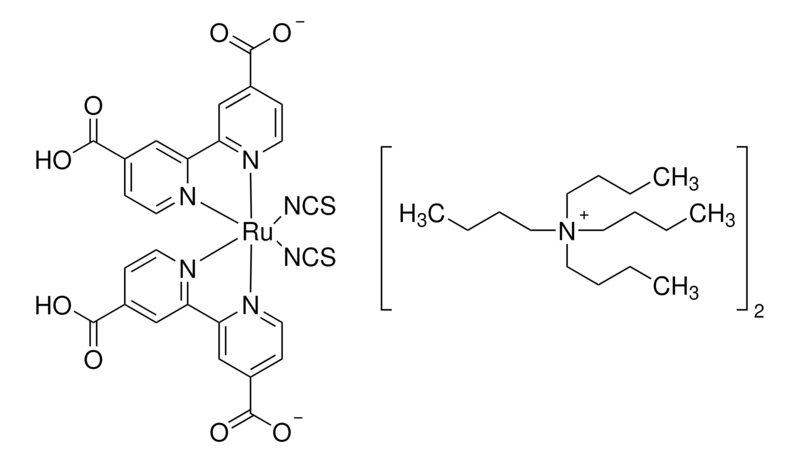
\includegraphics[width=0.6\textwidth]{n719.png}
		\caption{Wykorzystany barwnik N-719}
	\end{figure}
	
	\section{Zasada działania}
	Pełne działanie ogniwa DSSC tworzy cykl. W pierwszym kroku następuje wzbudzenie elektronu w barwniku ze stany HOMO do LUMO. Elektron ten jest następnie przenoszony na \ce{TiO2}, z którym barwnik jest w kontakcie. Elektron wydostaje się z ogniwa poprzez FTO i trafia do zewnętrznego układu. W elektrolicie zachodzi reakcja utleniania-redukcji \ce{3I^{-} -> I3^{-} + 2e-}. W produkcie jod ma stopień utlenienia $\frac{1}{3}$. Po drugiej stronie ogniwa wprowadzane są elektrony. Są one wykorzystywane do odwrócenia powyższej reakcji i odnowienia elektrolitu. Zamyka to pełen obwód. 
	\begin{figure}[H]
		\centering
		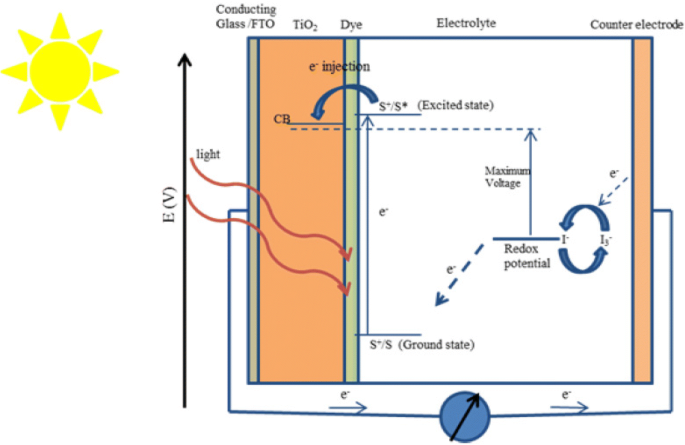
\includegraphics[width=\textwidth]{dssc.png}
		\caption{Schemat działania ogniwa DSSC \cite{dssc;fundamentals}}
	\end{figure}
	
	\section{Metoda wytwarzania}
	\subsection{Szkło z FTO}
	Szkło z FTO jest dostępne komercyjnie i nie jest wytwarzane na miejscu. Z większego kawałka wycinane są kwadraty o boku \qty{20}{\mm}. Na każde ogniwo potrzebne są dwa szkiełka i są one numerowane po stronie szkła. Sa one następnie czyszczone. Typowo pierwszym krokiem jest mycie specjalistycznym mydłem w celu usunięcia tłuszczu. Tym razem jednak ten krok pominięto, ponieważ jest on czasochłonny, a samo szkło było świeżo odpakowane i nie zostało jeszcze zanieczyszczone. Następnie w myjce ultradźwiękowej przeprowadzono dwa czyszczenie. W tym celu szkiełka umieszczono w osobnym zbiorniki z wydzielonymi miejscami na nie w celu uniknięcia stykania się ich ze sobą. Pierwsze czyszczenie było w acetonie przez \qty{20}{\min}. Po jego zakończeniu wymieniono aceton w zbiorniku na izopropanol i kontynuowano czyszczenie przez kolejne \qty{90}{\min}. Gdy już zakończono je szkiełka zostały przedmuchane sprężonym powietrzem, aby pozbyć się resztek izopropanolu i odstawiono do wyschnięcia. Ostatnim krokiem było naświetlanie szkiełek przy pomocy UV. Zostawiono je następnie do następnego dnia. 
	
	\subsection{Warstwa blokująca \ce{TiO2}}
	Pierwszym krokiem w przygotowaniu warstwy jest naklejenie na warstwę FTO taśmy Scotch w celu wydzielenia późniejszej elektrody. Wykorzystuje się tą taśmę, ponieważ nie pozostawia ona resztek kleju. Warstwa \ce{TiO2} została nałożona metodą spincoatera statycznie, to jest najpierw nałożono roztwór, a następnie obracano próbkę z prędkością \qty{1200}{\rpm} przez \qty{20}{\s}. Wykorzystano roztwór \ce{TiO2} w IPA w stosunku $1:9$. Z próbek zdjęto taśmę, aby uniknąć jej uszkodzenia, a następnie wygrzewano w temperaturze \qty{400}{\degreeCelsius} przez \qty{15}{\min}. Po tym czasie zostały one zdjęte do ochłodzenia. 
	\begin{figure}[H]
		\centering
		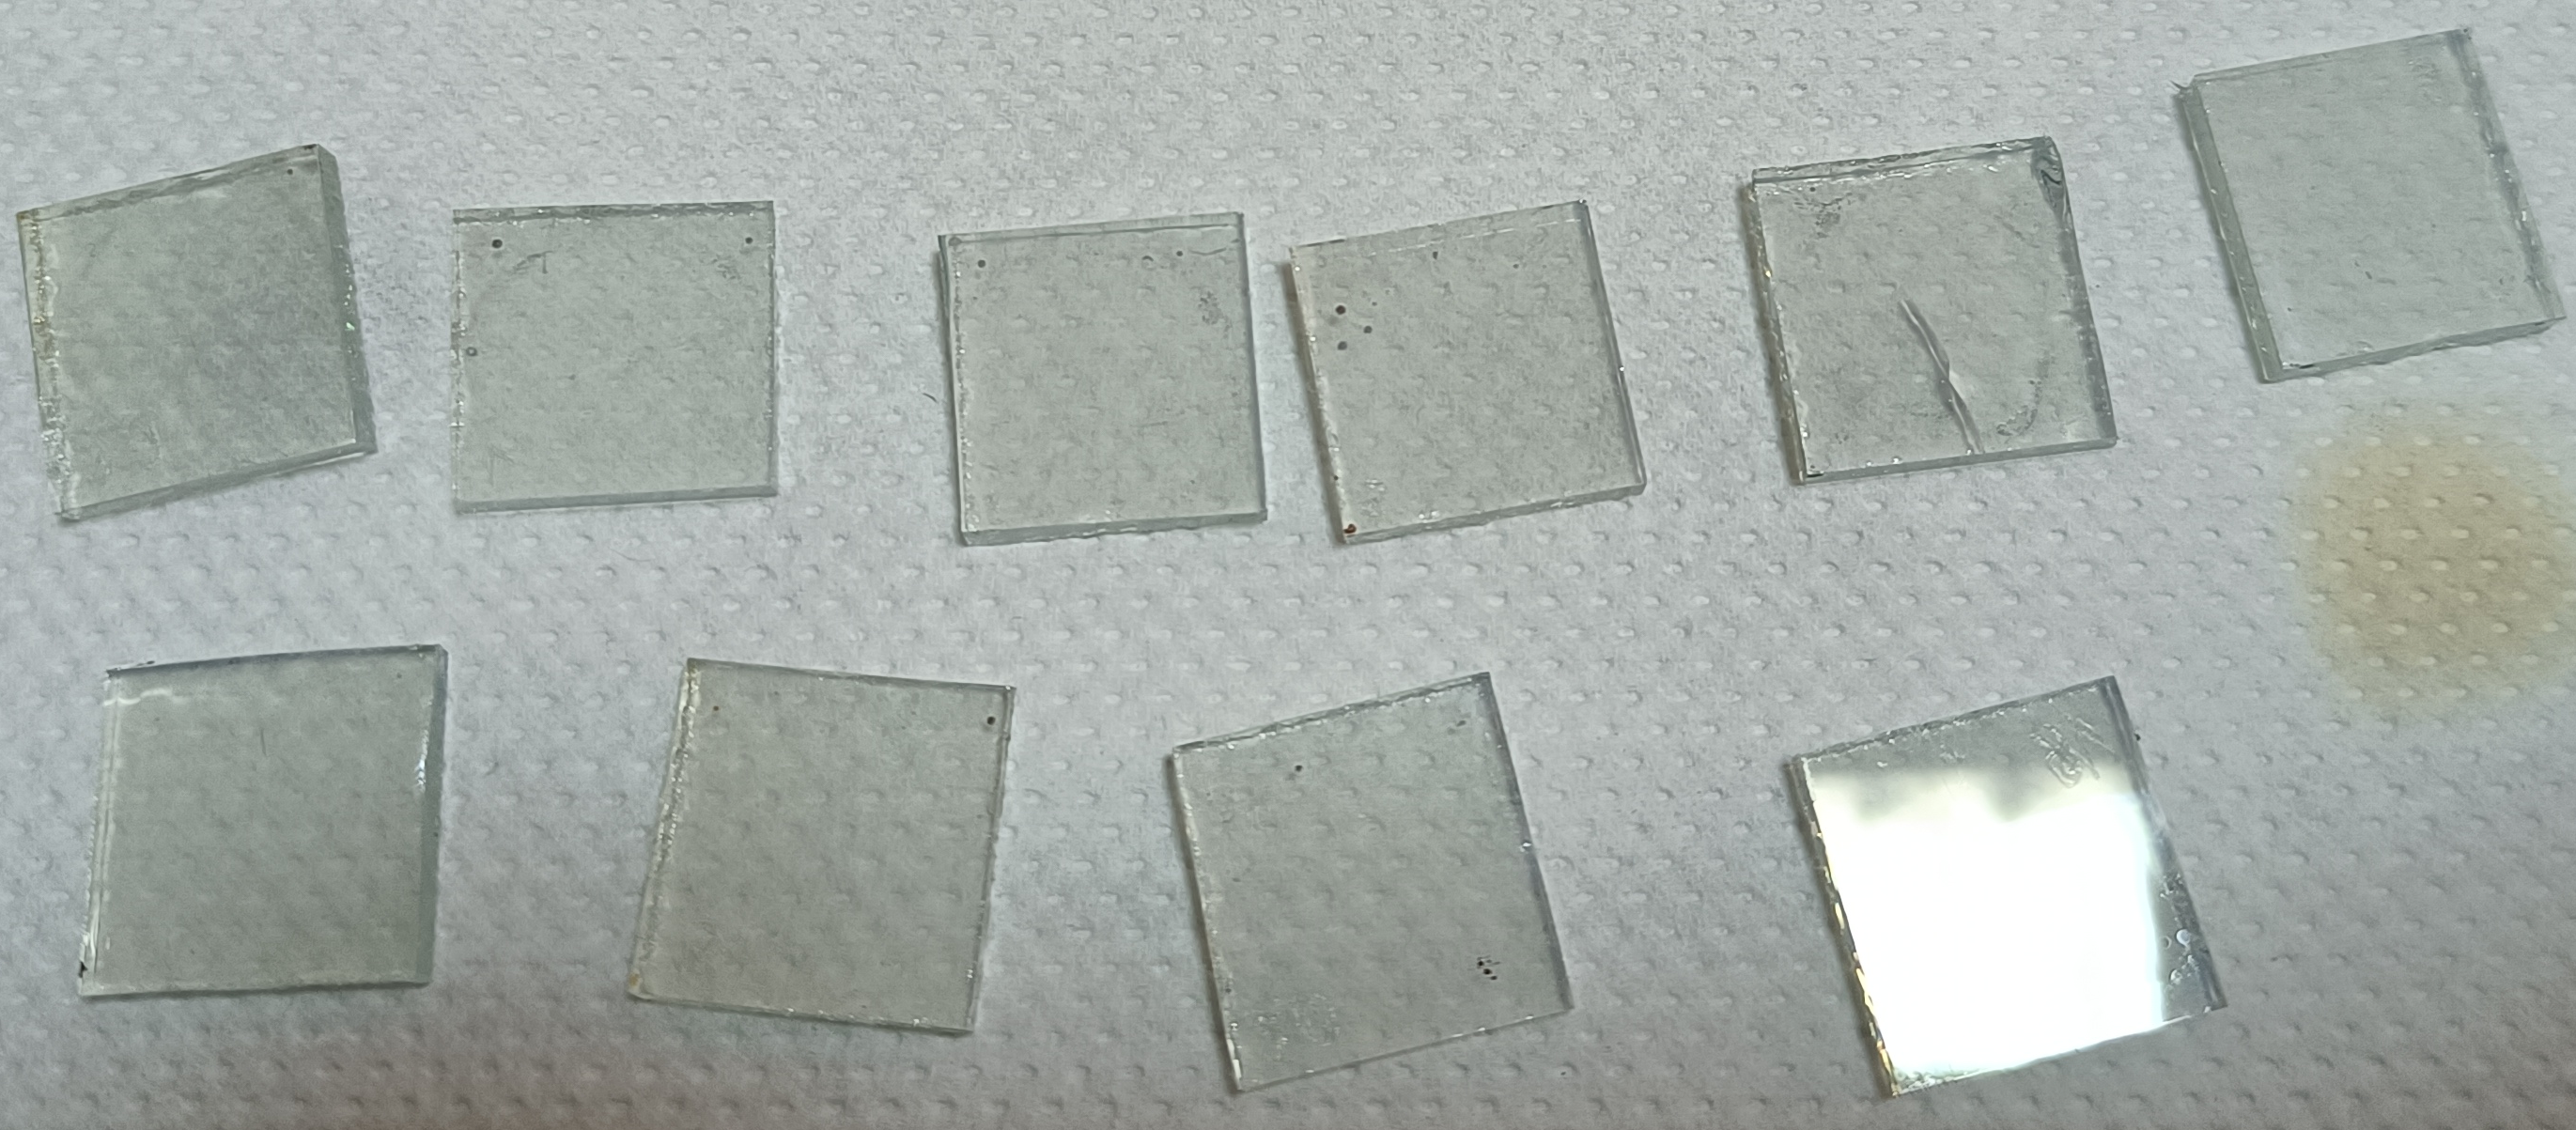
\includegraphics[width=0.6\textwidth]{probki_tio2_blok.png}
		\caption{Próbki po nałożeniu warstwy blokującej \ce{TiO2}; jest ona widoczna jedynie pod pewnymi kątami}
	\end{figure}
	
	\subsection{Warstwa porowata \ce{TiO2}}
	W pierwszej kolejności naklejono nową taśmę w taki sposób, aby wydzielona powierzchnia w całości znajdowała się na warstwie blokującej. Ma to na celu uniknięcie kontaktu między elektrolitem a FTO; zmniejszenie powierzchni nie ma znaczenia dla funkcjonowania ogniwa. Wykorzystano metodę rakli (ang. doctor blade, właściwie ductor blade). W tym celi na wydzieloną powierzchnię próbki nałożono kropelkę pasty z zawiesiną nanocząstek \ce{TiO2}. Nadmiar pasty został zdjęty poprzez przesunięcie szkiełkiem mikroskopowym po powierzchni. Grubość warstwy jest ograniczona otaczającą obszar aktywny taśmą. Następnie zdjęto taśmę i wygrzano próbki w temperaturze \qty{500}{\degreeCelsius} przez \qty{30}{\min}. Podobnie jak poprzednio po tym czasie odstawiono je do ochłodzenia. 
	\begin{figure}[H]
		\centering
		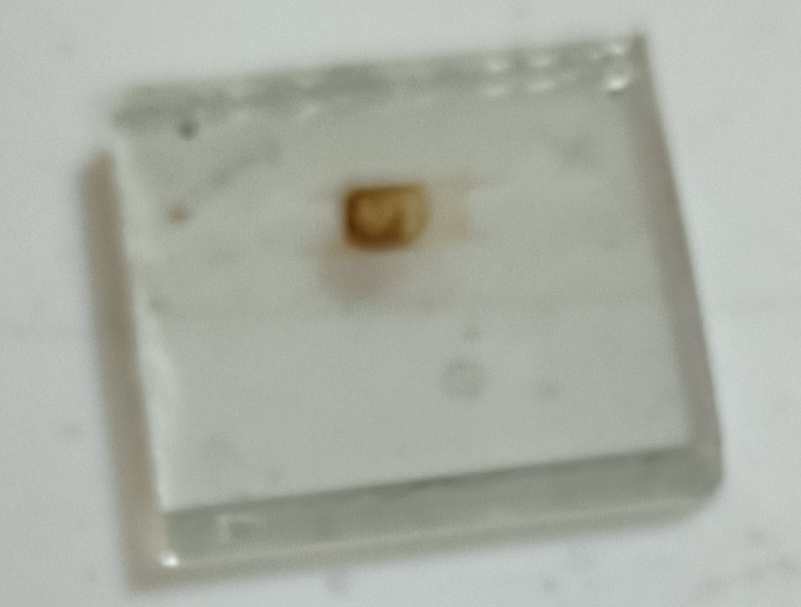
\includegraphics[width=0.6\textwidth]{probki_tio2_poro.png}
		\caption{Próbka po nałożeniu warstwy porowatej \ce{TiO2}; widoczna jest wydzielona powierzchnia ogniwa}
	\end{figure}
	
	\subsection{Warstwa barwnika}
	Próbki zanurzono w roztworze N-719 w etanolu i zostawiono je w nim przez kilkanaście godzin. Porowata struktura \ce{TiO2} znacznie zwiększa powierzchnię kontaktu, przez to większa ilość barwnika jest w stanie się na nim osadzić. Następnego dnia po wyjęciu próbek z roztworu zostały one przemyte etanolem z nadmiaru barwnika. Pełna nazwa N-719 to Di-tetrabutylammonium cis-bis(isothiocyanato)bis(2,2'-bipyridyl-4,4'-dicarboxylato)ruthenium(II)
	\begin{figure}[H]
		\centering
		\begin{subfigure}{0.45\textwidth}
			\centering
			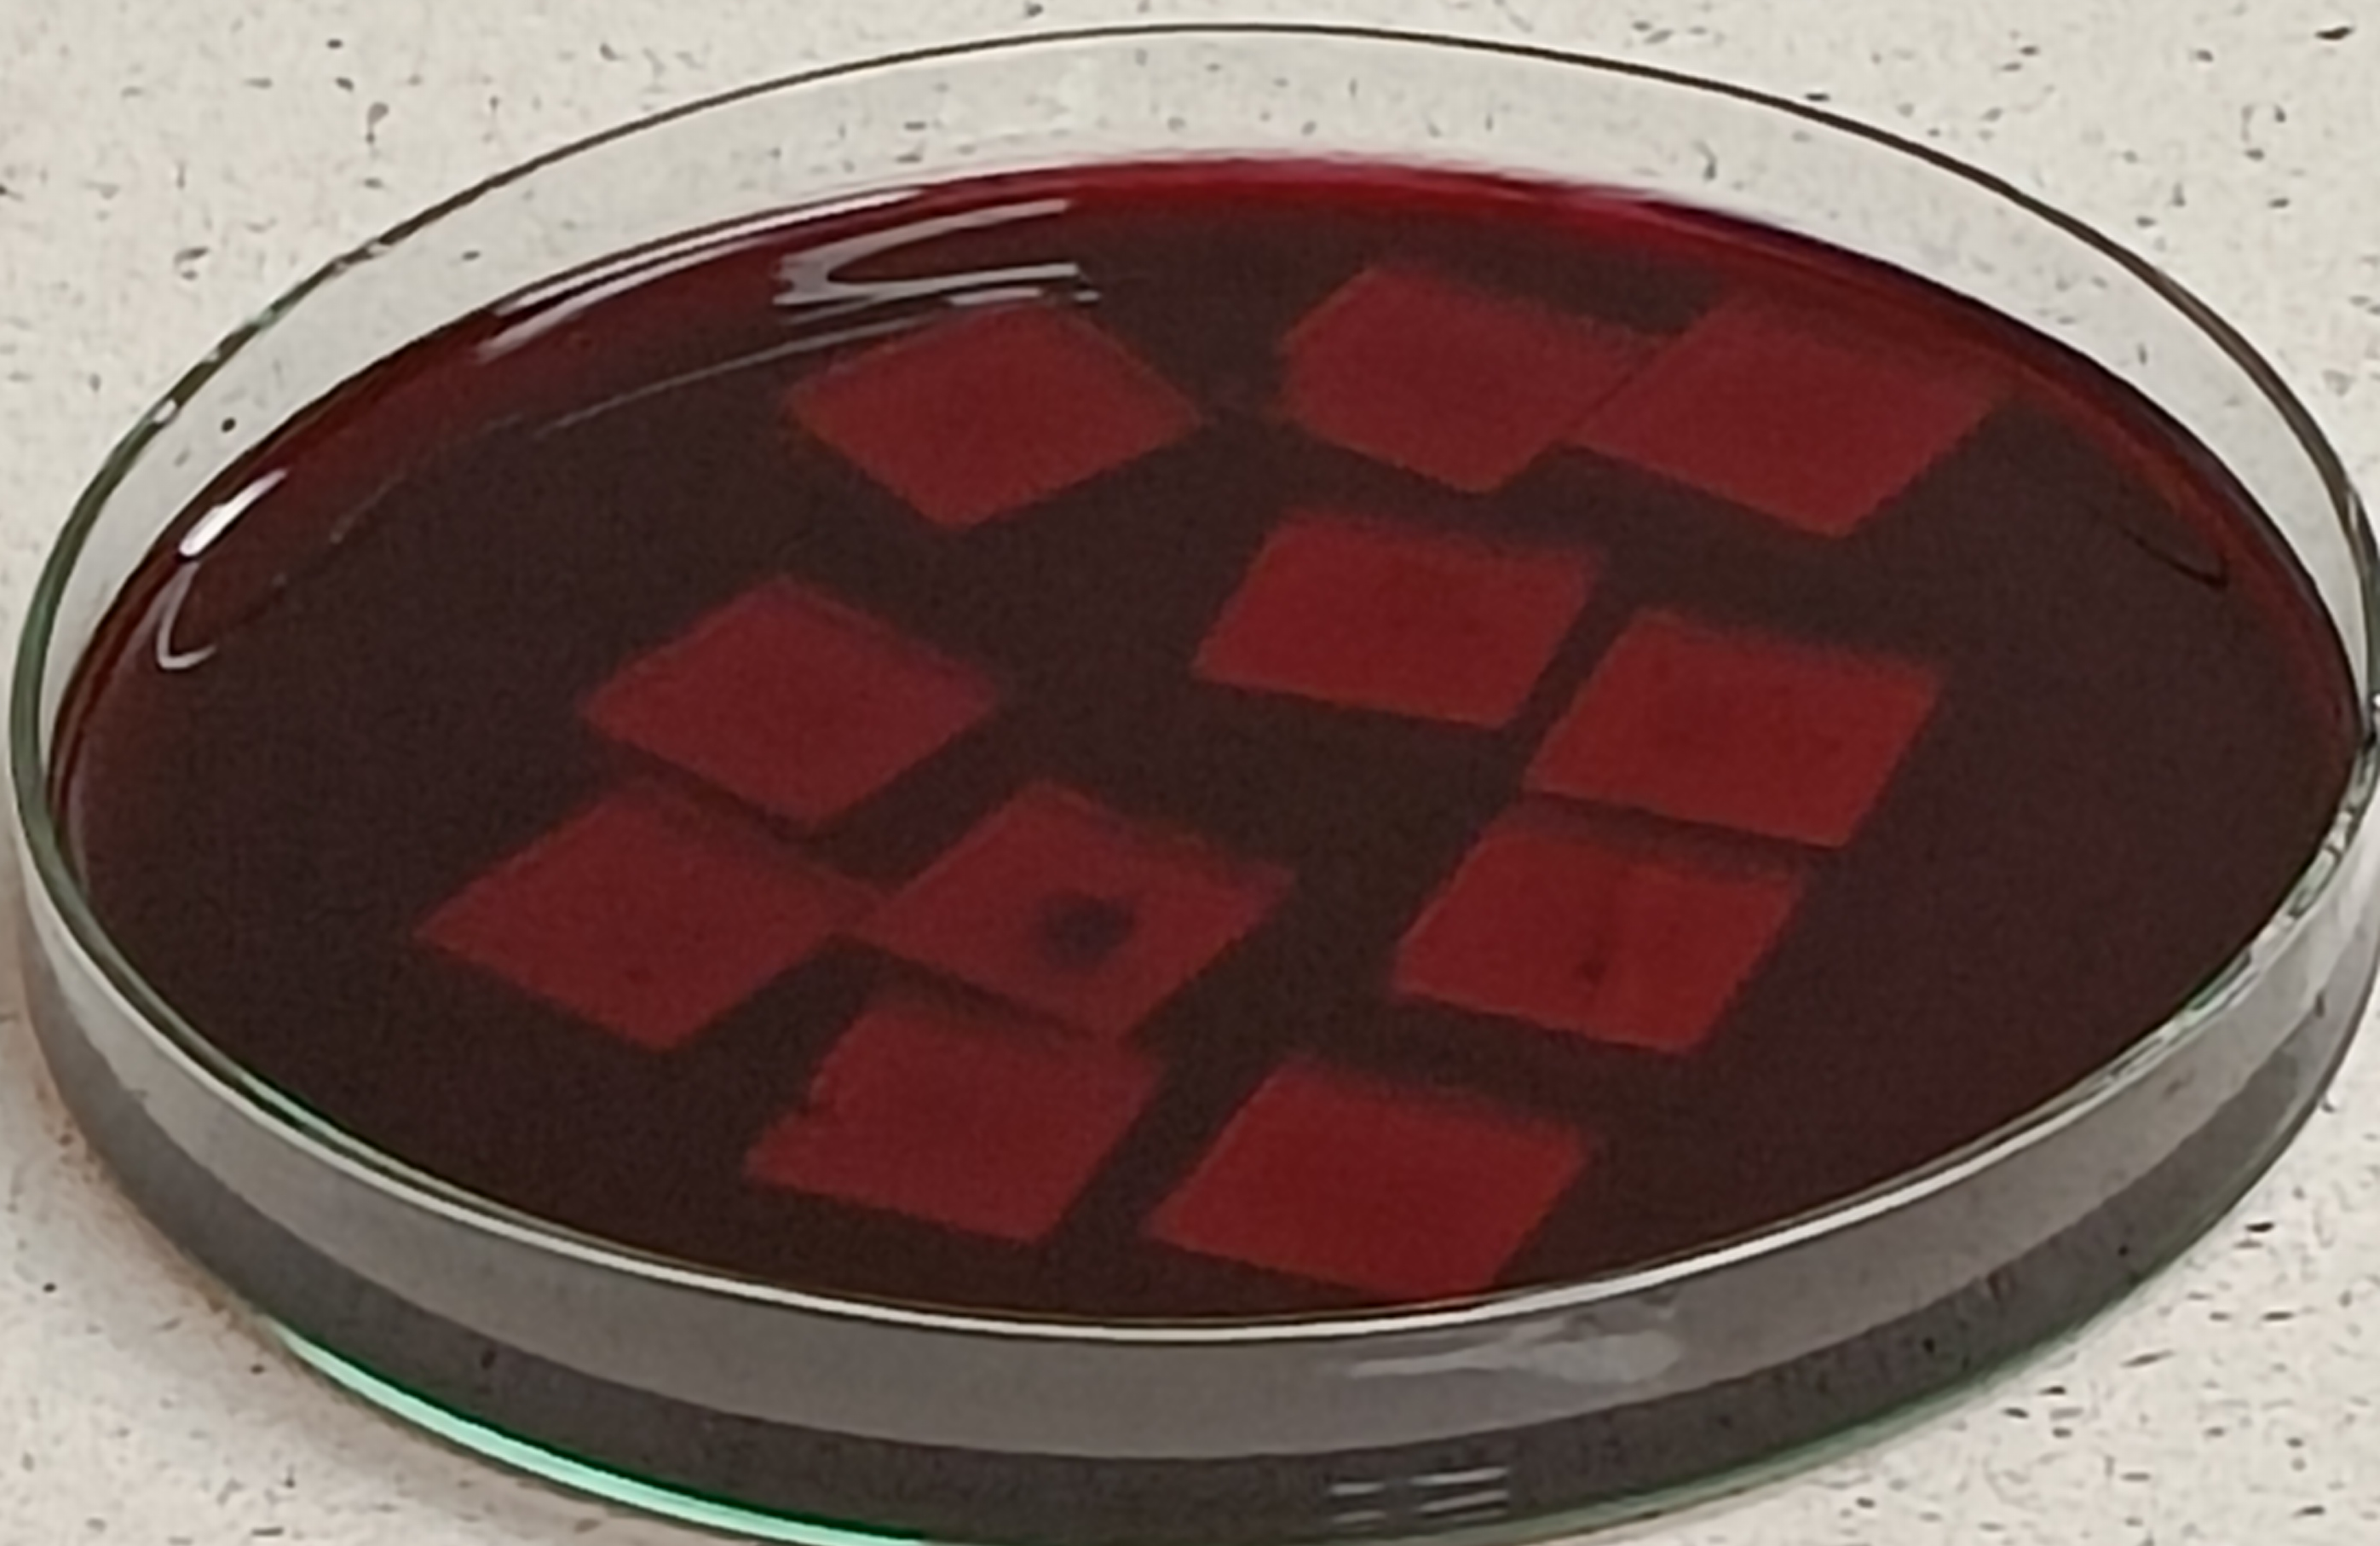
\includegraphics[width=\textwidth]{probki_w_barwniku_przed.png}
			\caption{\label{fig:barwnik_przed}}
		\end{subfigure}
		\begin{subfigure}{0.45\textwidth}
			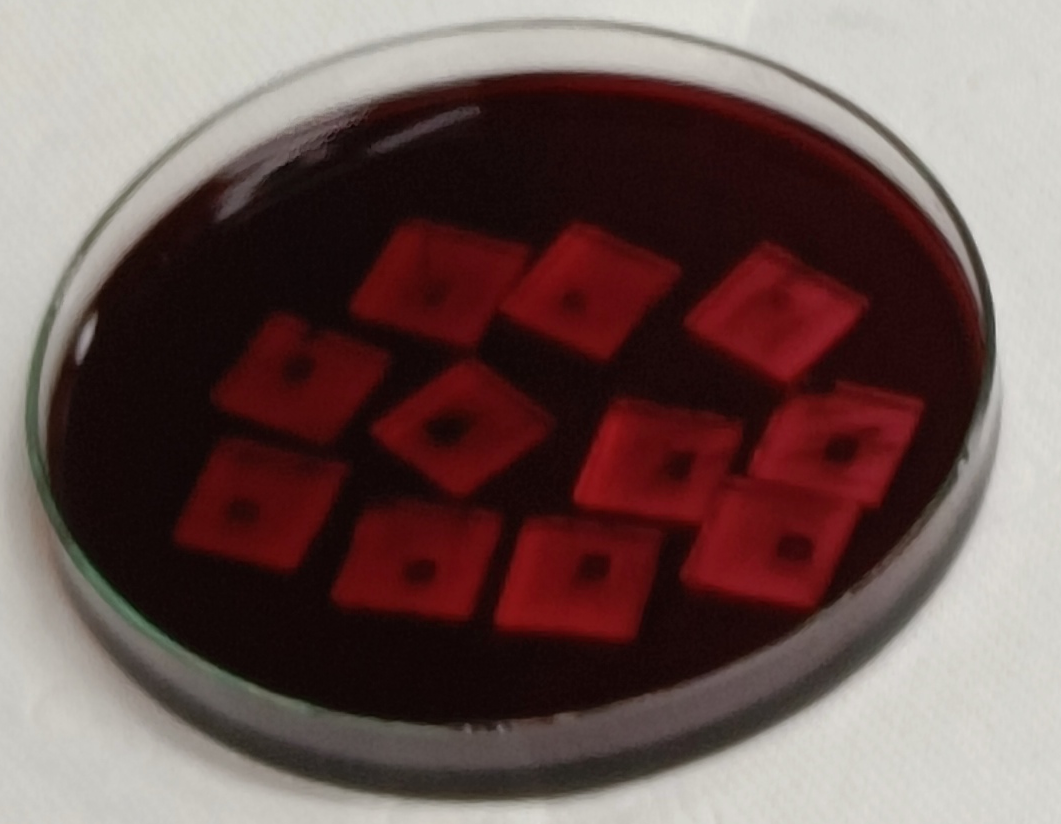
\includegraphics[width=\textwidth]{probki_w_barwniku_po.png}
			\caption{\label{fig:barwnik_po}}
		\end{subfigure}
		\captionsetup{subrefformat=parens}
		\caption{Próbki w barwniku: \subref{fig:barwnik_przed} przed i \subref{fig:barwnik_po} po kąpieli w barwniku.}
	\end{figure}
	
	\subsection{Warstwa platyny}
	Jedyną warstwą nałożoną na drugie szkiełko jest platyna. Tworzy to przeciwelektrodę. Warstwa FTO nie jest tu ściśle wymagana, dlatego nie ma potrzeby używania taśmy w celu wydzielenia podłączenia do FTO, ale połączenie będzie bezpośrednie do platyny. Wykorzystano metodę kroplową (ang. drop casting) z roztworem platyny. Wytwarzanie wielu ze szkiełek przeprowadzono inną metodą, gdzie temperatura była zmienna w zakresie \qtyrange{100}{500}{\degreeCelsius}. Dla wyższych temperatur występował efekt Leidenfrosta, gdzie rozpuszczalnik wrzał gwałtownie na granicy kropli i szkła tworząc izolującą granicę pary. Uniemożliwiało to równomierne rozprowadzenie roztworu na powierzchni. 
	\begin{figure}[H]
		\centering
		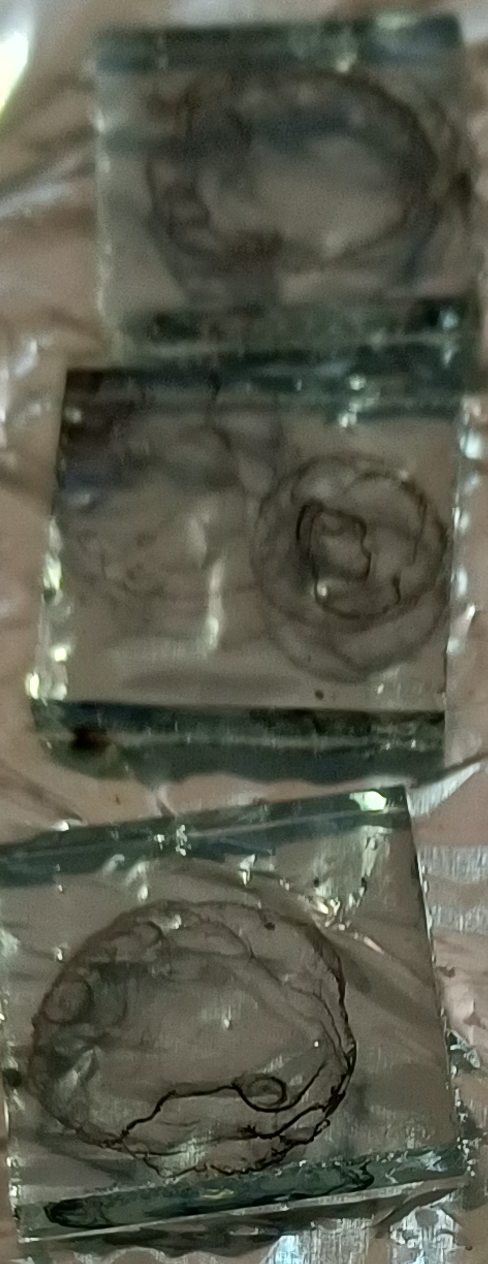
\includegraphics[angle=90, width=0.7\textwidth]{probki_platyna.png}
		\caption{Warstwa platyny na szkle}
	\end{figure}
	
	\section{Charakterystyka otrzymanych ogniw}
	
	
	\subsection{Ogniwo numer 1}
	\begin{figure}[H]
		\centering
		\begin{tikzpicture}
			\begin{axis}[scale only axis,
				width=0.8\textwidth,
				xlabel=$U\;\bab{\unit{\mV}}$,
				ylabel=$I\;\bab{\unit{\uA}}$,
				grid=both,
				xmin=0,
				xmax=300,
				ymin=0,
				ymax=5,
				xtick distance=50,
				ytick distance=1,
				minor tick num=4,
				legend pos=south west]
				\addplot [color=red  , smooth, mark=*, mark size=1.5pt] table [x=UmV, y=IuA] {barw_1_sorted.txt};
			\end{axis}
		\end{tikzpicture}
		\caption{Zależność prądu od napięcia}
		\label{fig:barw_1_i}
	\end{figure}
	\begin{figure}[H]
		\centering
		\begin{tikzpicture}
			\begin{axis}[scale only axis,
				width=0.8\textwidth,
				xlabel=$U\;\bab{\unit{\mV}}$,
				ylabel=$P\;\bab{\unit{\nW}}$,
				grid=both,
				xmin=0,
				xmax=300,
				ymin=0,
				ymax=400,
				xtick distance=50,
				ytick distance=100,
				minor tick num=4,
				legend pos=south west]
				\addplot [color=red  , smooth, mark=*, mark size=1.5pt] table [x=UmV, y=PnW] {barw_1_sorted.txt};
			\end{axis}
		\end{tikzpicture}
		\caption{Zależność mocy od napięcia}
		\label{fig:barw_1_p}
	\end{figure}
	\begin{table}[H]
		\centering
		\begin{tabular}{
				S[table-column-width=1.5cm]
				S[table-column-width=1.5cm]
				S[table-column-width=1.5cm]
				S[table-column-width=1.5cm]
				S[table-column-width=1.5cm]
				S[table-column-width=1.5cm]}
			\toprule
			{\makecell{$U_{OC}$ \\ $\bab{\unit{\mV}}$}} & 
			{\makecell{$I_{SC}$ \\ $\bab{\unit{\uA}}$}} & 
			{\makecell{$U_{MPP}$ \\ $\bab{\unit{\mV}}$}} & 
			{\makecell{$I_{MPP}$ \\ $\bab{\unit{\uA}}$}} & 
			{\makecell{FF \\ $\bab{\unit{\percent}}$}} & 
			{\makecell{$P_{MPP}$ \\ $\bab{\unit{\nW}}$}} \\
			\midrule
			%Uoc    Isc   Umpp    Impp  FF     Pmpp
			281.0 & 4.0 & 158.3 & 1.9 & 26.8 & 300.77 \\
			\bottomrule
		\end{tabular}
		\caption{Parametry ogniwa}
	\end{table}
	
	\subsection{Ogniwo numer 9}
	\begin{figure}[H]
		\centering
		\begin{tikzpicture}
			\begin{axis}[scale only axis,
				width=0.8\textwidth,
				xlabel=$U\;\bab{\unit{\mV}}$,
				ylabel=$I\;\bab{\unit{\uA}}$,
				grid=both,
				xmin=0,
				xmax=600,
				ymin=0,
				ymax=40,
				xtick distance=50,
				ytick distance=5,
				minor tick num=4,
				legend pos=south west]
				\addplot [color=red  , smooth, mark=*, mark size=1.5pt] table [x=UmV, y=IuA] {barw_9_sorted.txt};
			\end{axis}
		\end{tikzpicture}
		\caption{Zależność prądu od napięcia}
		\label{fig:barw_9_i}
	\end{figure}
	\begin{figure}[H]
		\centering
		\begin{tikzpicture}
			\begin{axis}[scale only axis,
				width=0.8\textwidth,
				xlabel=$U\;\bab{\unit{\mV}}$,
				ylabel=$P\;\bab{\unit{\nW}}$,
				grid=both,
				xmin=0,
				xmax=600,
				ymin=0,
				ymax=5,
				xtick distance=50,
				ytick distance=1,
				minor tick num=4,
				legend pos=south west]
				\addplot [color=red  , smooth, mark=*, mark size=1.5pt] table [x=UmV, y=PuW] {barw_9_sorted.txt};
			\end{axis}
		\end{tikzpicture}
		\caption{Zależność mocy od napięcia}
		\label{fig:barw_9_p}
	\end{figure}
	\begin{table}[H]
		\centering
		\begin{tabular}{
				S[table-column-width=1.5cm]
				S[table-column-width=1.5cm]
				S[table-column-width=1.5cm]
				S[table-column-width=1.5cm]
				S[table-column-width=1.5cm]
				S[table-column-width=1.5cm]}
			\toprule
			{\makecell{$U_{OC}$ \\ $\bab{\unit{\mV}}$}} & 
			{\makecell{$I_{SC}$ \\ $\bab{\unit{\uA}}$}} & 
			{\makecell{$U_{MPP}$ \\ $\bab{\unit{\mV}}$}} & 
			{\makecell{$I_{MPP}$ \\ $\bab{\unit{\uA}}$}} & 
			{\makecell{FF \\ $\bab{\unit{\percent}}$}} & 
			{\makecell{$P_{MPP}$ \\ $\bab{\unit{\uW}}$}} \\
			\midrule
			%Uoc    Isc    Umpp    Impp   FF     Pmpp
			597.6 & 37.2 & 273.9 & 18.1 & 22.3 & 4.96 \\
			\bottomrule
		\end{tabular}
		\caption{Parametry ogniwa}
	\end{table}
	
	\subsection{Ogniwo numer 13}
	\begin{figure}[H]
		\centering
		\begin{tikzpicture}
			\begin{axis}[scale only axis,
				width=0.8\textwidth,
				xlabel=$U\;\bab{\unit{\mV}}$,
				ylabel=$I\;\bab{\unit{\uA}}$,
				grid=both,
				xmin=0,
				xmax=800,
				ymin=0,
				ymax=120,
				xtick distance=100,
				ytick distance=40,
				minor tick num=4,
				legend pos=south west]
				\addplot [color=red  , smooth, mark=*, mark size=1.5pt] table [x=UmV, y=IuA] {barw_13_sorted.txt};
			\end{axis}
		\end{tikzpicture}
		\caption{Zależność prądu od napięcia}
		\label{fig:barw_13_i}
	\end{figure}
	\begin{figure}[H]
		\centering
		\begin{tikzpicture}
			\begin{axis}[scale only axis,
				width=0.8\textwidth,
				xlabel=$U\;\bab{\unit{\mV}}$,
				ylabel=$P\;\bab{\unit{\uW}}$,
				grid=both,
				xmin=0,
				xmax=800,
				ymin=0,
				ymax=40,
				xtick distance=100,
				ytick distance=10,
				minor tick num=4,
				legend pos=south west]
				\addplot [color=red  , smooth, mark=*, mark size=1.5pt] table [x=UmV, y=PuW] {barw_13_sorted.txt};
			\end{axis}
		\end{tikzpicture}
		\caption{Zależność mocy od napięcia}
		\label{fig:barw_13_p}
	\end{figure}
	\begin{table}[H]
		\centering
		\begin{tabular}{
				S[table-column-width=1.5cm]
				S[table-column-width=1.5cm]
				S[table-column-width=1.5cm]
				S[table-column-width=1.5cm]
				S[table-column-width=1.5cm]
				S[table-column-width=1.5cm]}
			\toprule
			{\makecell{$U_{OC}$ \\ $\bab{\unit{\mV}}$}} & 
			{\makecell{$I_{SC}$ \\ $\bab{\unit{\uA}}$}} & 
			{\makecell{$U_{MPP}$ \\ $\bab{\unit{\mV}}$}} & 
			{\makecell{$I_{MPP}$ \\ $\bab{\unit{\uA}}$}} & 
			{\makecell{FF \\ $\bab{\unit{\percent}}$}} & 
			{\makecell{$P_{MPP}$ \\ $\bab{\unit{\uW}}$}} \\
			\midrule
			%Uoc    Isc     Umpp    Impp   FF     Pmpp
			753.4 & 108.9 & 583.0 & 56.0 & 39.8 & 32.65 \\
			\bottomrule
		\end{tabular}
		\caption{Parametry ogniwa}
	\end{table}
	
	\subsection{Ogniwo numer 20}
	\begin{figure}[H]
		\centering
		\begin{tikzpicture}
			\begin{axis}[scale only axis,
				width=0.8\textwidth,
				xlabel=$U\;\bab{\unit{\mV}}$,
				ylabel=$I\;\bab{\unit{\uA}}$,
				grid=both,
				xmin=0,
				xmax=800,
				ymin=0,
				ymax=800,
				xtick distance=100,
				ytick distance=100,
				minor tick num=4,
				legend pos=south west]
				\addplot [color=red  , smooth, mark=*, mark size=1.5pt] table [x=UmV, y=IuA] {barw_20_sorted.txt};
			\end{axis}
		\end{tikzpicture}
		\caption{Zależność prądu od napięcia}
		\label{fig:barw_20_i}
	\end{figure}
	\begin{figure}[H]
		\centering
		\begin{tikzpicture}
			\begin{axis}[scale only axis,
				width=0.8\textwidth,
				xlabel=$U\;\bab{\unit{\mV}}$,
				ylabel=$P\;\bab{\unit{\uW}}$,
				grid=both,
				xmin=0,
				xmax=800,
				ymin=0,
				ymax=400,
				xtick distance=100,
				ytick distance=100,
				minor tick num=4,
				legend pos=south west]
				\addplot [color=red  , smooth, mark=*, mark size=1.5pt] table [x=UmV, y=PuW] {barw_20_sorted.txt};
			\end{axis}
		\end{tikzpicture}
		\caption{Zależność mocy od napięcia}
		\label{fig:barw_20_p}
	\end{figure}
	\begin{table}[H]
		\centering
		\begin{tabular}{
				S[table-column-width=1.5cm]
				S[table-column-width=1.5cm]
				S[table-column-width=1.5cm]
				S[table-column-width=1.5cm]
				S[table-column-width=1.5cm]
				S[table-column-width=1.5cm]}
			\toprule
			{\makecell{$U_{OC}$ \\ $\bab{\unit{\mV}}$}} & 
			{\makecell{$I_{SC}$ \\ $\bab{\unit{\uA}}$}} & 
			{\makecell{$U_{MPP}$ \\ $\bab{\unit{\mV}}$}} & 
			{\makecell{$I_{MPP}$ \\ $\bab{\unit{\uA}}$}} & 
			{\makecell{FF \\ $\bab{\unit{\percent}}$}} & 
			{\makecell{$P_{MPP}$ \\ $\bab{\unit{\uW}}$}} \\
			\midrule
			%Uoc    Isc     Umpp    Impp    FF     Pmpp
			642.0 & 703.1 & 488.9 & 685.1 & 74.2 & 334.95 \\
			\bottomrule
		\end{tabular}
		\caption{Parametry ogniwa}
	\end{table}
	
	\section{Bibliografia}
	\printbibliography
\end{document}